\section{Introduction}
Segmenting demonstrations of a multistep task is an important first step in a number of robot learning applications: skill-learning \cite{calinon2010learning, kruger2010learning, konidaris2011robot}, learning from demonstrations \cite{Niekum2015learning}, reward function parametrization \cite{hanlearning}, and automation of surgical subtasks \cite{murali2015learning}.
One approach is manual annotation, which can be time-consuming and error-prone if inconsistent.
Therefore, it is desirable to algorithmically extract segments from unlabled data.
Such algorithms fall into two broad categories: (1) dictionary-based, (2) and unsupervised.
Dictionary-based algorithms set a pre-defined vocabulary of primitives \emph{a priori} and decompose new trajectories in terms of the primitives; and this approach has been widely applied in the analysis of robotic surgery \cite{lea15improved,zappella2013surgical}.

However, the key challenge in using a dictionary-based approach is building the dictionary of primitives. 
Overly specific primitives may not cover all of the actions seen in a set of demonstrations, while overly general primitives may miss task-specific structure.
Unsupervised techniques can avoid dependence on a pre-defined set of primitives.
Unsupervised methods typically assume some generative mixture model for the data, e.g., locally Gaussian segments, and fit trajectories to this model grouping together locally similar points \cite{calinon2010learning, krishnan2015tsc, calinon2004stochastic, kruger2010learning, fox2009nonparametric, oh2005learning}.


\begin{figure}[ht]
\centering
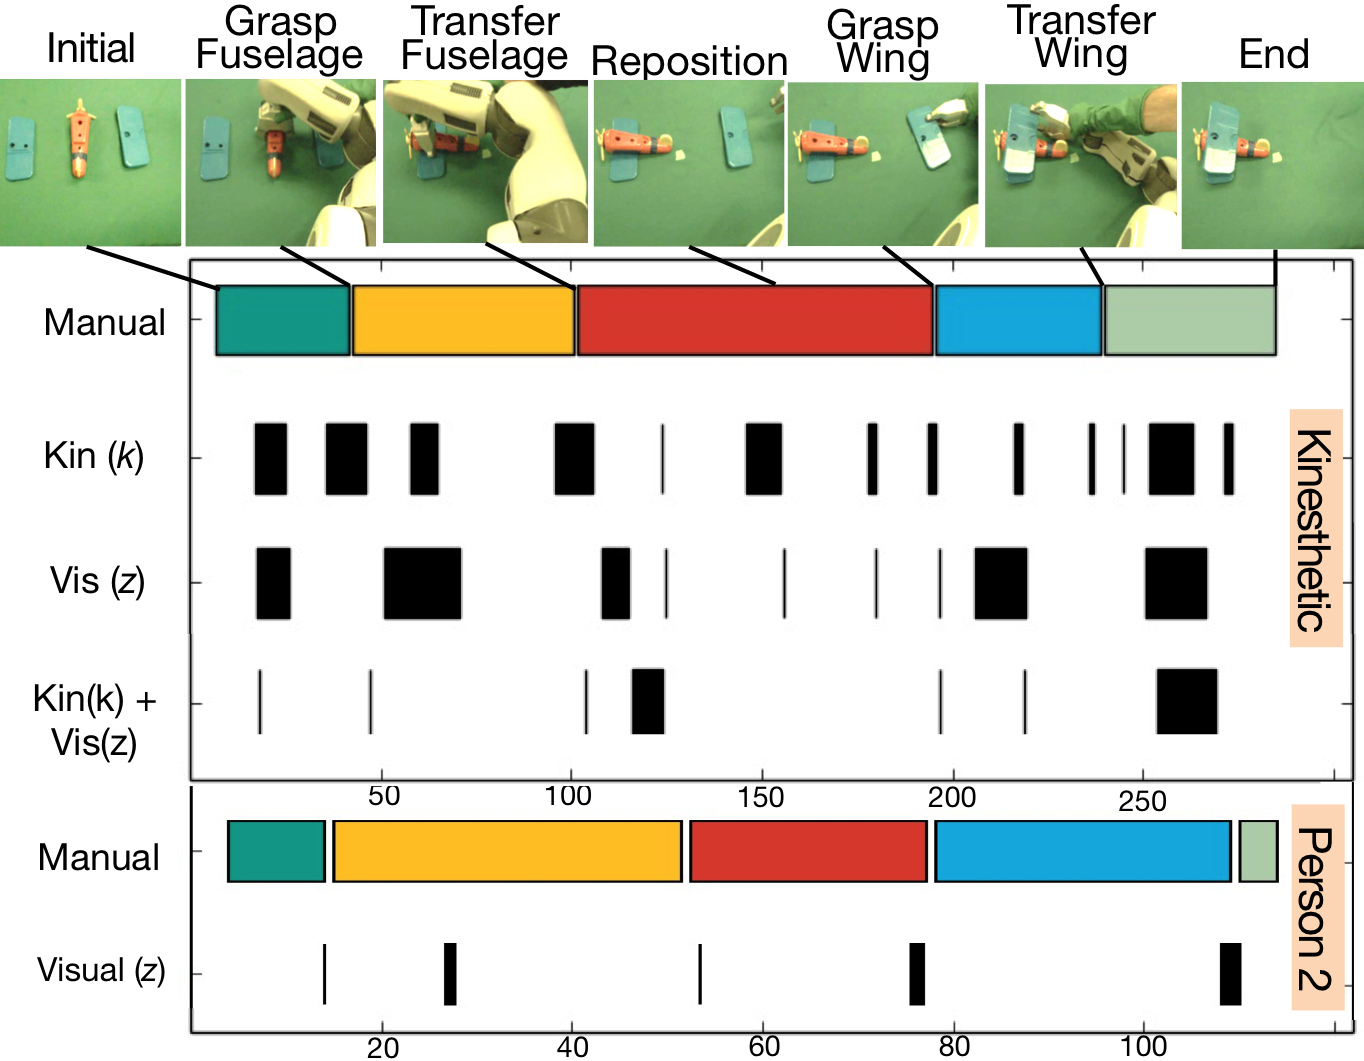
\includegraphics[width=\linewidth]{figures/pr2_plane_assembly.png}
\caption{The figure shows a sequence of images from the Toy Plane assembly (YCB Dataset). The first row shows a manual segmentation of the task in 4 semantic steps: Grasp Fuselage, Transfer Fuselage, Grasp Wing, Transfer Fuselage. Rows 2-4 show the sub-task level segmentation results from our completely unsupervised approach using 8 examples. Each row is a sequence of transitions represented by blocks. The width of every block represents the confidence interval conveying the length of transition, with some transitions being sharp while others are longer.}
 \label{fig:pr2_toyplane}
\vspace{-10pt} 
\end{figure}

While unsuperivsed segmentation has been widely studied in the context of kinematic data segmentation, increasingly, fixed camera video recordings accompany kinematic recordings of human teleoperation in a variety of datasets \cite{hodgins2009guide, gao2014jigsaws, ofli2013berkeley}.
The importance of visual sensing in segmentation has been suggested by experimental results in our prior work \cite{krishnan2015tsc} and by others \cite{Niekum2015learning}.
Visual features can provide crucial information in a number of scenarios: (1) a robot can only partially observe its state with kinematic data, (2) state-dependent sensor noise in a robots kinematic data, and (3) manipulations of objects in the environment.
However, existing unsupervised approaches rely on highly constrained visual sensing models: hand tuned features \cite{krishnan2015tsc}, poses for all objects in the workspace via AR markers \cite{Niekum2015learning}, or motion capture markers in human gesture extraction \cite{kulic2011incremental}.

In this work, we explore how we can relax these constraints by segmenting both kinematics and natural videos of demonstrations.
The key problem is leveraging raw visual data, i.e., pixels, due to the dimensionality and the featurization problem.
Fortunately, in computer vision, the growing maturity of \emph{deep} featurization e.g., Convolutional Neural Networks (CNNs), has led to a number of seminal results in visual feature extraction \cite{krizhevsky2012imagenet, lecun1995convolutional, jia2014caffe, long2014fully}.
Furthermore, frameworks like CAFFE \cite{jia2014caffe} allow for sharing pre-trained models (on terabyte-scale corpora of natural images), and this allows us to take advantage of these results even with relatively small datasets.

We explore an extension (\sys) to the Transition State Clustering algorithm \cite{krishnan2015tsc} with visual features.
At a high-level, this algorithm models demonstrations as switched linear dynamical systems.
It then identifies states at which regime transitions occur and clusters these states to identify regions of the state space associated with transitions.
The minimal covering set of transition clusters, i.e., clusters representing all demonstrations, gives a semantic segmentation for a task. 
We extend this framework by specifying the state space not only with kinematic states but also augmented with visual features.
Our experimental results surprisingly suggest that a time-series of frame-level visual features behave almost like smooth kinematic trajectories--satisfying the assumptions in our prior work.
Even with featurized videos, segmentation is not trivial, and there are a number of open questions including how to incorporate visual features into the model, how to navigate the number of hyperparameter and architecture choices, and the sufficiency of pre-trained networks.

We summarize the key experimental results.

\vspace{0.25em}

\textbf{Q0. Do generic visual features, deep or otherwise, improve segmentation accuracy? } While prior work in segmentation establishes that features from a constrained/hand-annotated visual sensing model can improve segmentation, an open question is whether there is enough information in natural videos with general-purpose features to improve segmentation accuracy. Our experimental results find that under partial kinematic observation and sensing noise, visual features dramatically improve segmentation accuracy by \textbf{x\%???}.

\vspace{0.25em}

\textbf{Q1. How do we transfer pre-trained neural network features to a very different domain? } Transfer learning of convolutional neural networks is an open problem in the computer vision community and a number of recent publications suggest caution or highly sensitive results \cite{oquab2014learning}.  These networks are trained on very different corpora of images than those seen in robotic demonstration videos. Even so, our results suggest that with the appropriate choice of convolutional layer to transfer, we can achieve accuracy improvements of \textbf{x\%???}.

\vspace{0.25em}

\textbf{Q2. How should visual features be incorporated into a kinematic segmentation model? } Even with automated featurization, the visual feature space is much higher dimensional than the kinematic state space. We explore dimensionality reduction techniques to mitigate some challenges due to the dimensionality. A natural approach would be to treat this problem as a multi-view manifold alignment problem e.g., finding a feature space maximally correlated with kinematics with Canonical Correlation Analysis. Surprisingly, our results suggest that this approach discards the novel information discovered by vision, and in fact random projections would do just as well (\textbf{x\%???}).

\vspace{0.25em}

\textbf{Q3. How do learned segmentations compare with human annotations? } We apply \sys to data from two datasets of surgical tasks \cite{gao2014jigsaws} where there were also human annotations of the same tasks.
While we find that \sys mostly agrees with the human annotations, there are a number of instances where \sys find crucial actions missed by the human annotators. (\textbf{List examples}) 

\iffalse
\begin{figure}[ht]
\centering
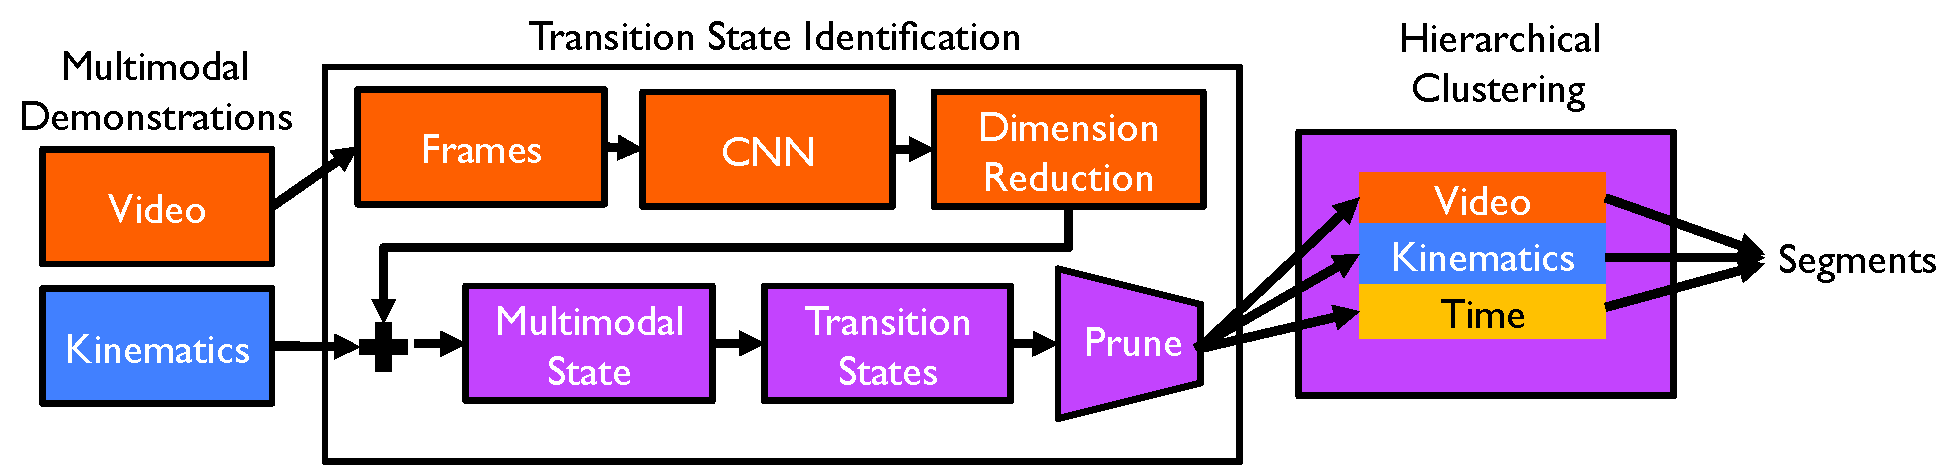
\includegraphics[width=\columnwidth]{figures/architecture.pdf}
\caption{\todo{name} architecture. We use a pre-trained CNN to featurize raw video data for use in segmentation. After featurization, we combine the data with kinematic data and apply a Transition State Clustering algorithm to identify segments. \label{fig:arch}}
\vspace{-1em}
\end{figure}
\fi
